\documentclass[../../main.tex]{subfiles}

\begin{document}

\section{Transformers}
\subsection{Introduction}

The Transformer \parencite{vaswani2017attention} is a deep learning model that has been revolutionary in the field of machine learning. Originally devised as a sequence-to-sequence model that uses attention to learn the relationships between the input and output sequences. Transformers have been the state of the start in the field of natural language processing (NLP) leading to the development of models like BERT \parencite{devlin2019bert} and GPT \parencite{brown2020language}. As of recent, they are gaining traction in fields like computer vision \parencite{dosovitskiy2021image} becoming the new state of the art in a field that has been dominated by Convolutional Neural Networks (CNNs). The attractiveness of transformers stems from their general purpose nature and strong ability to learn relationships with a large context window whilst being massively parallelizable. A brief overview of the transformer model is given below.


\subsection{Embedding}

Data points it into a vector representation called an \emph{embedding} or \emph{token} ensuring positional information is added to these tokens via a positional encoding. The embedding is a simple linear transformation of the input data $\bm{X} \elof{N}{D}$ where $N$ is the number of data points and $D$ is the dimensionality of the data. 

\subsection{Self-Attention}

 Self-attention is the key component of the transformer model. It is a way to learn the relationships between the data in the input sequence itself.  Consider a language modelling task, the sentence \texttt{The quick brown fox jumps over the lazy dog} has strong attention between the data like \texttt{fox} and \texttt{jumps} representing an action, \texttt{brown} and \texttt{fox} representing the color of the fox and so on, then there are very weak attentions between data \texttt{quick} and \texttt{dog} representing the lack of relationship between the two data. Using self-attention we can learn these relationships between the data in the input sequence, giving a powerful mechanism to learn the relationships.

In the transformer models we will use the embeddings $\bm{X} \elof{N}{D}$ as the input to generate a query $\bm{Q} \elof{N}{d_k}$, a key $\bm{K} \elof{N}{d_k}$ and a value $\bm{V} \elof{N}{d_v}$ matrices via a simple linear transformation matrix $\bm{W_q} \elof{D}{d_k}$, $\bm{W_k} \elof{D}{d_k}$ and $\bm{W_v} \elof{D}{d_v}$ respectively. 

Where each row of the matrices is the query, key and value vectors for each data point in the input sequence. 

The query, key and value matrices are then used to compute the attention matrix $\bm{A} \elof{N}{N}$ as follows:

\begin{equation}
    \bm{A} = \text{softmax}\left(\frac{\bm{Q}\bm{K}^T}{\sqrt{d_k}}\right)
\end{equation}

\noi The intuition is to compute the similarity between the query and the key vectors using dot product between the query and key vectors. The softmax is used to normalize the attention matrix so that the rows sum to 1. The softmax is also scaled by $\sqrt{d_k}$ to prevent the softmax from saturating. The attention matrix is then used to compute the output matrix $\bm{H} \elof{N}{d_v}$ as $\bm{H} = \bm{A}\bm{V}$

The overall attention function for a layer is given by:

\begin{equation}
    \bm{H} =\text{Attention}(\bm{Q}, \bm{K}, \bm{V}) = \text{softmax}\left(\frac{\bm{Q}\bm{K}^T}{\sqrt{d_k}}\right)\bm{V}
\end{equation}

\subsection{Multi-Head Self-Attention}

Currently, the attention matrix $\bm{A}$ is computed once so the model only learns one attention relationship, however, we can take advantage of using multiple attention `heads' in parallel to learn many attention relationships, this scheme is called the \emph{Multi-Head Attention} (MHSA). 

Each attention head is computed using simple dot product attention of a transformed query, key and value matrix. They are transformed by a simple linear layer (a matrix) which is unique for each head of the MHSA, $\bm{W_q}\isup{i} \elof{d_k}{d_k}$, $\bm{W_k}\isup{i} \elof{d_k}{d_k}$ and $\bm{W_v}\isup{i} \elof{d_v}{d_v}$ where $i \in [1, h]$ for a head count of $h$. Then the attention for the particular head is computed as follows:

\begin{equation}
	\bm{H}\isup{i} = \text{Attention}(\bm{Q}\bm{W_q}\isup{i}, \bm{K}\bm{W_k}\isup{i}, \bm{V}\bm{W_v}\isup{i}) \elof {N}{d_v}
\end{equation}

The output of the MHSA is the concatenation of the outputs of each head $\bm{H}\isup{i}$ (stacked on to of each other) multiplied by a learnable matrix $\bm{W_O} \elof{hd_v}{D}$ which transforms the concatenated output to the original dimensionality of the input sequence.

\begin{align*}
	 \text{MHSA}(\bm{Q}, \bm{K}, \bm{V}) &= \text{cat}(\bm{H}\isup{1}; \bm{H}\isup{2}; \dots; \bm{H}\isup{h})\bm{W_O} 
	= \begin{bmatrix}
		\bm{H}\isup{1} \\
		\bm{H}\isup{2} \\
		\vdots \\
		\bm{H}\isup{h}
	\end{bmatrix} \bm{W_O} \elof{N}{D}
\end{align*}

% The figure below summarizes the MHSA operation.

% \begin{figure}[H]
% 	\centering
% 	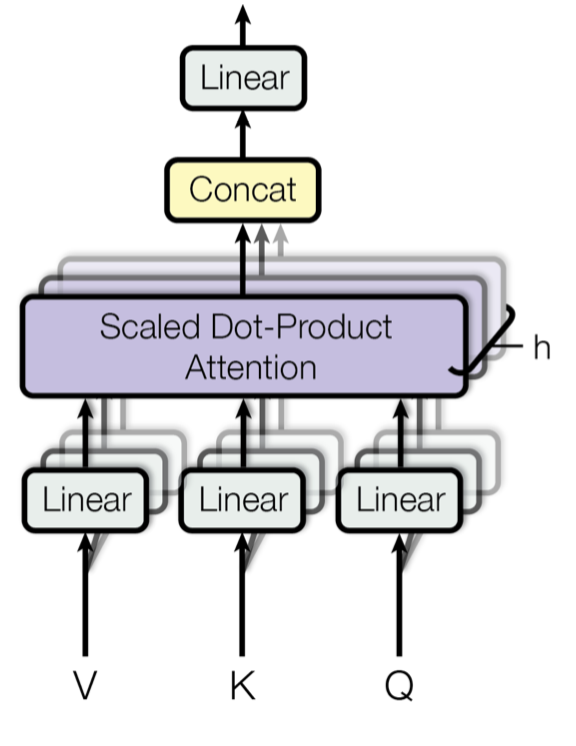
\includegraphics[height=0.4\textwidth]{./mhsa.png}
% 	\caption{Multi-Head Self-Attention \parencite{vaswani2017attention}}
% \end{figure}

\subsection{Encoder}

\begin{figure}[H]
	\centering
	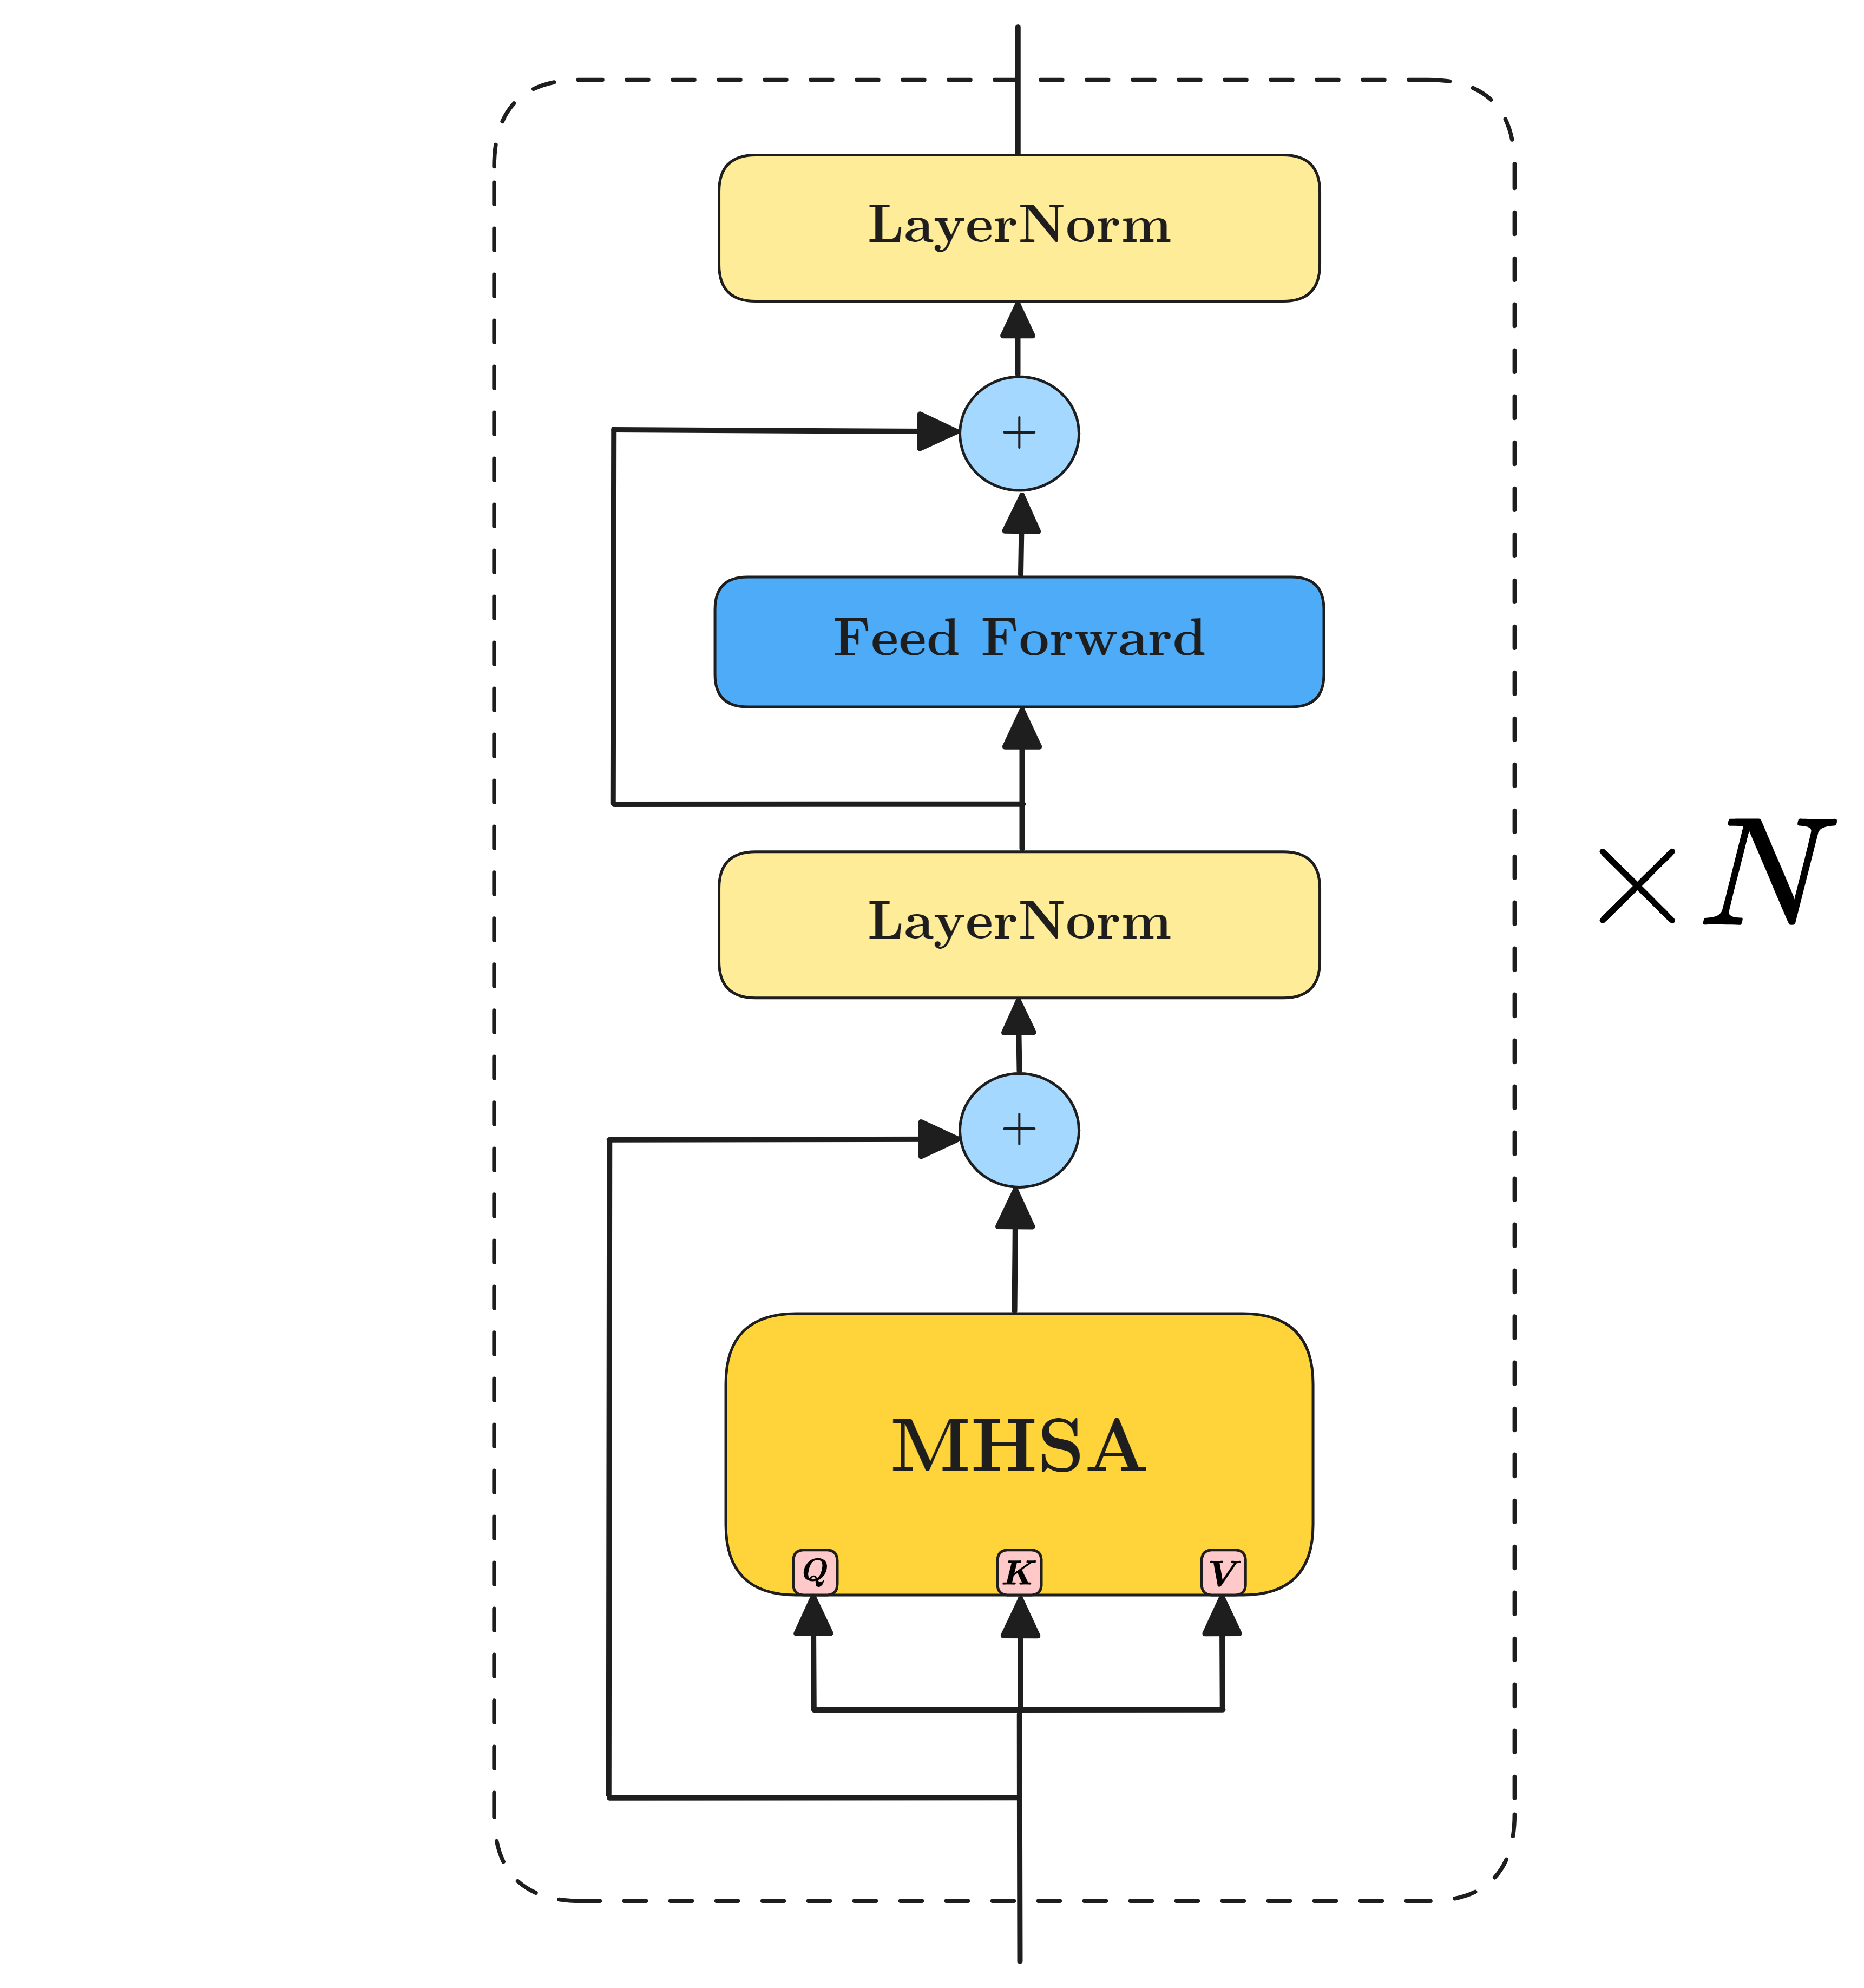
\includegraphics[height=0.5\textwidth]{./encoder.png}
	\caption{Transformer Encoder \parencite{vaswani2017attention}}
	\label{fig:encoder}
\end{figure}

\autoref{fig:encoder} shows the encoder of the transformer model. The encoder is composed of a stack of $N$ identical layers. Each layer is composed of two sub-layers, the MHSA and a simple feed-forward network. The output of each sub-layer is passed through a residual connection and a layer normalization operation \parencite{ba2016layer}. The final output of the encoder is the output of the last layer which shall be denoted as $\bm{Y} \elof{N}{D}$. 

\begin{note}[Key Points]

The Transformer Encoder Layer takes an input set of embeddings $\bm{X} \elof{N}{D}$ and outputs a set of embeddings $\bm{Y} \elof{N}{D}$ of the \textbf{same dimensionality} but with the \textbf{patterns of the input sequence learned}. It can be viewed as a function that takes a set and outputs a set of the same dimensionality.

\end{note}

\ifSubfilesClassLoaded{%
    \printbibliography{}
}{} 


\end{document}